\documentclass{beamer}
\usepackage[utf8]{inputenc}
\usetheme{Boadilla}
\usecolortheme{seahorse}
\usepackage[french]{babel}
%\usepackage{kpfonts}
\usepackage{tikz}

\usepackage{amsmath} % load the AMS math package
\usefonttheme{professionalfonts} % use the same font for math as in regular LaTeX document
\usepackage{unicode-math} % load a Unicode math font package
%\setmathfont{Latin Modern Math}



\title[ML]{ML Projet}
\author{Isai Gordeev}
\institute{École Polytechnique}
\date{\today}

\begin{document}
	
	\begin{frame}
		\titlepage
	\end{frame}
	
	\begin{frame}
		\frametitle{Plan}
			\tableofcontents
	
	\end{frame}


	\section{ML ou pas?}
	
	
	\begin{frame}
		\frametitle{ML ou pas?}
		\begin{center}
			Vous êtes sûr en emploi de ML?\\
			Votre problème peut être résolu \textbf{algorithmiquement}
		\end{center}
		
	\end{frame}

	\subsection{Oui, je suis sûr et alors quoi?}
		\begin{frame}
		\frametitle{Oui, je suis sûr et alors quoi?}
		\centering
		ML essaie de trouver une fonction f tel que
		$$f(X) = y$$
		$$ {\displaystyle f(X):=f^{L}(W^{L}f^{L-1}(W^{L-1}\cdots f^{1}(W^{1}x)\cdots ))} $$
		
		où X est notre attributs, y est caractéristique
		
		\begin{figure}
			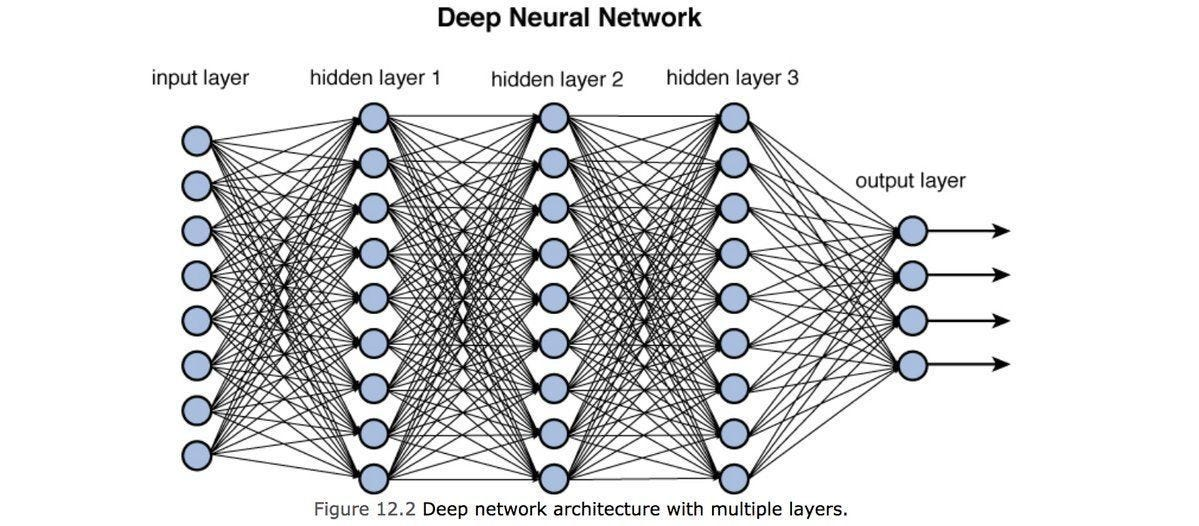
\includegraphics[width=0.8\textwidth]{neuron}
			\label{fig:example}
		\end{figure}
		
	\end{frame}


	\section{Architecture}
	
	\begin{frame}
		\frametitle{Architecture}
		\begin{itemize}
			\item Réseau neuronal convolutif (CNN) – le traitement des images
			\item Réseaux antagonistes génératifs (GAN) - la génération des objets
			\item Transformer – l'architecture d'utilisation générale
		\end{itemize}
		
		\begin{columns}[c]
			\column{.3\textwidth}
			\centering
			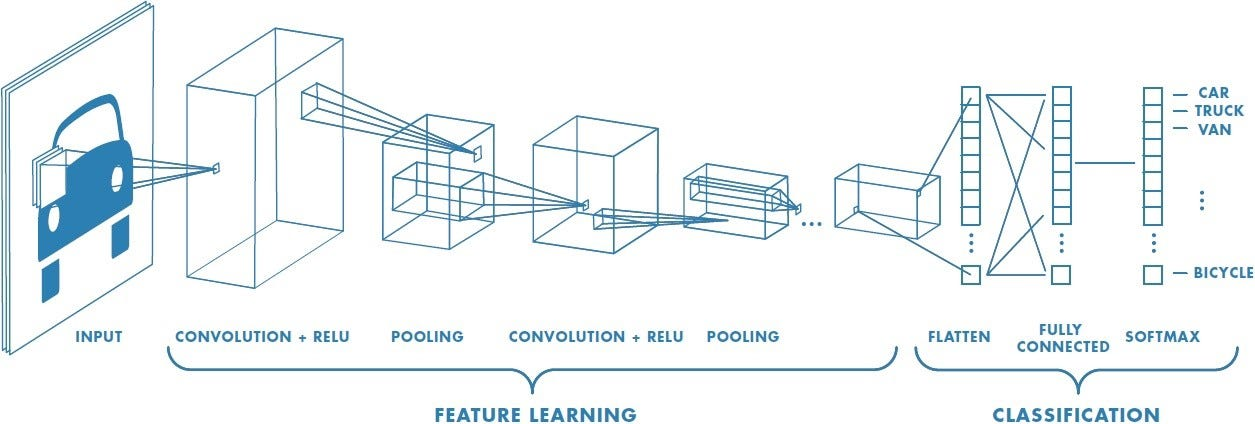
\includegraphics[width=\textwidth]{3}
			\column{.3\textwidth}
			\centering
			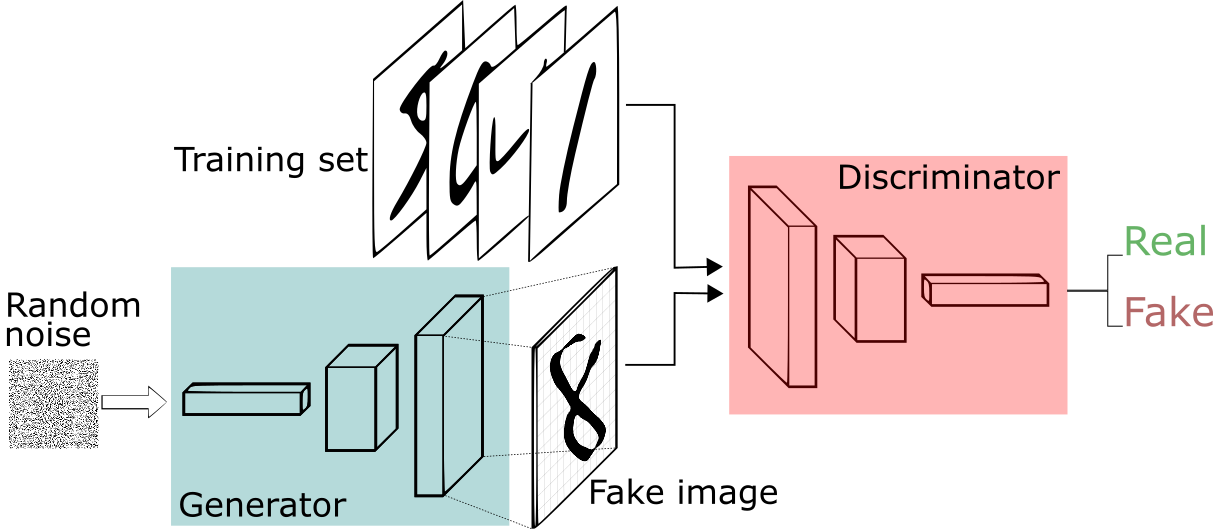
\includegraphics[width=\textwidth]{2}
			\column{.3\textwidth}
			\centering
			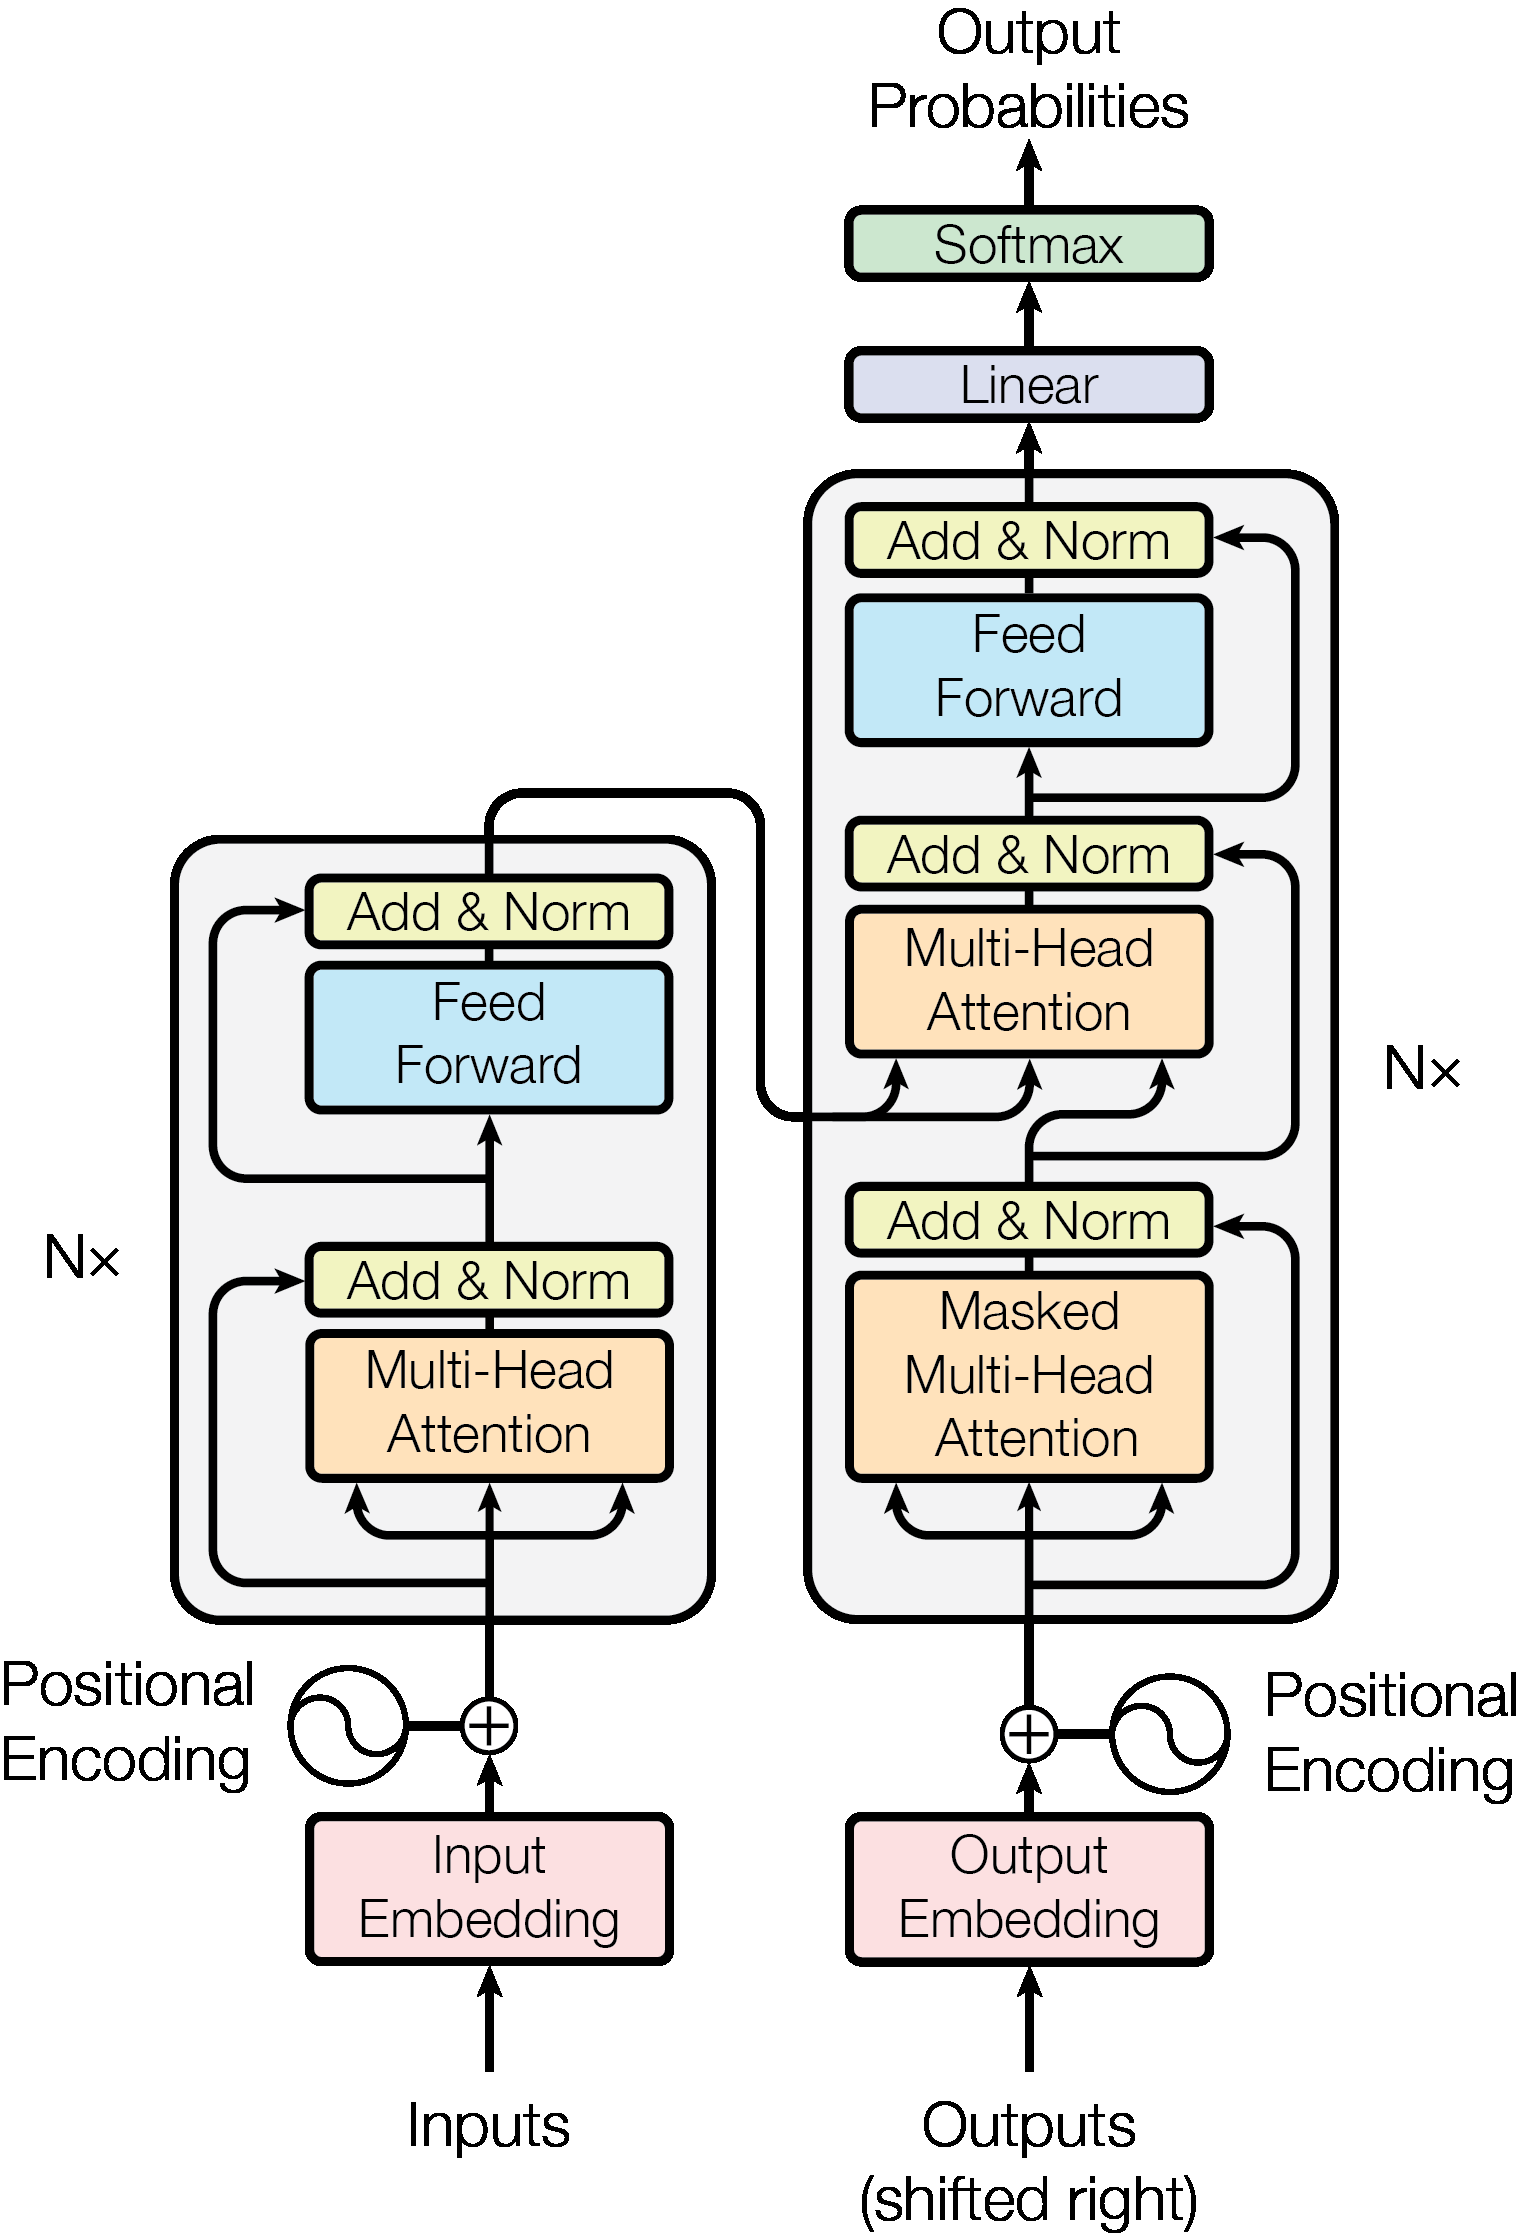
\includegraphics[width=\textwidth]{1}
		\end{columns}
	
	
	\end{frame}

	\section{Metaparaméters}

\begin{frame}
	\frametitle{Metaparaméters}
	\begin{itemize}
		\item Le réseau
		\begin{itemize}
			\item Les fonctions d'activations
			\item Les couches
			\item Autres
		\end{itemize}
	\item Vraisemblance
	\begin{itemize}
		\item La fonction de perte $L(W, y, \hat y)$
		\item Régularization 
		\item Autres
	\end{itemize}
	\end{itemize}

			
	\begin{columns}[c]
		\column{.3\textwidth}
		\centering
		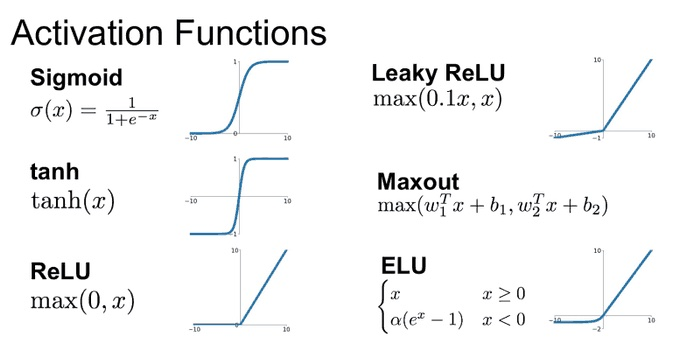
\includegraphics[width=\textwidth]{5}
		\column{.3\textwidth}
		\centering
		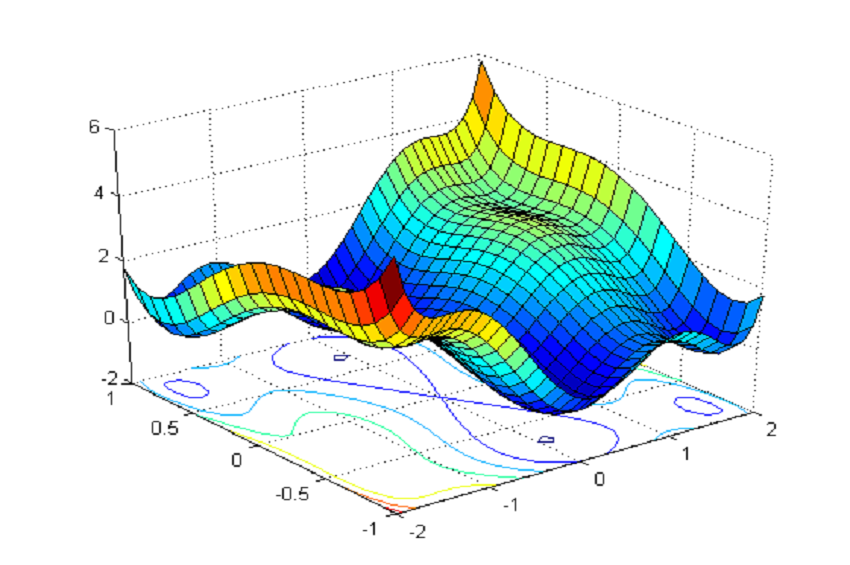
\includegraphics[width=\textwidth]{4}
		\column{.3\textwidth}
		\centering
		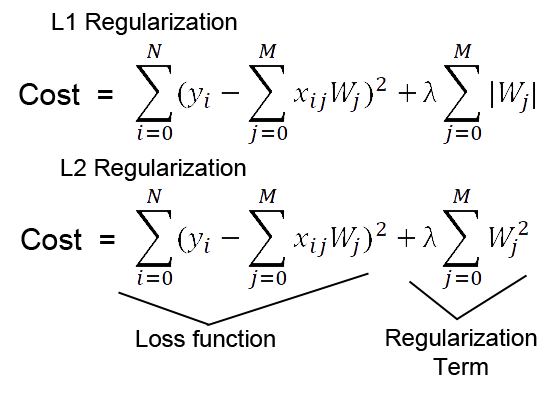
\includegraphics[width=\textwidth]{6}
	\end{columns}
\end{frame}
	
	\section{Données}

	\begin{frame}
		\frametitle{Données}
		\begin{itemize}
			\item Il faut collecter les données (ou notre tensor X)
			\item Il fait éviter les attributs dépendants
			\item Pour l'apprentissage 80\% de données
			\item Pour la validation 20\% de données
		\end{itemize}
	
		\begin{center}
			Par exemple on a n image de chat noir\\
			Il faut dire si une image contient un chat noir 
		\end{center}
	\end{frame}



		\section{Apprentissage}
	
	\begin{frame}
		\frametitle{Apprentissage}
		\begin{enumerate}
			\item Rétropropagation
		$$	{\displaystyle {\begin{aligned}\delta ^{1}&=(f^{1})'\circ (W^{2})^{T}\cdot (f^{2})'\circ \cdots \circ (W^{L-1})^{T}\cdot (f^{L-1})'\circ (W^{L})^{T}\cdot (f^{L})'\circ \nabla _{a^{L}}C\\\delta ^{2}&=(f^{2})'\circ \cdots \circ (W^{L-1})^{T}\cdot (f^{L-1})'\circ (W^{L})^{T}\cdot (f^{L})'\circ \nabla _{a^{L}}C\\&\vdots \\ \delta ^{L-1}&=(f^{L-1})'\circ (W^{L})^{T}\cdot (f^{L})'\circ \nabla _{a^{L}}C\\\delta ^{L}&=(f^{L})'\circ \nabla _{a^{L}}C,\end{aligned}}}
		$$
			
			\item Algorithme du gradient stochastique
			
			$$ W^i=W^i-\lambda \nabla L(W, y, \hat y)_{W^i} = W^i-\lambda \delta^i_W $$
			$$ L (W, y, \hat y) = arg( min_{X} L (W, y, \hat y))
		\end{enumerate}
	

	\end{frame}

	\section{Réglage}
	
	\begin{frame}
		\frametitle{Réglage}
		\centering 
		On maintient le modèle en répétant les étapes 3 - 5 (2 - 5) \\

	

\begin{tikzpicture}[node distance=1.5cm,auto]
	\tikzstyle{block} = [rectangle, draw=blue, thick, fill=blue!20,    text width=3.5cm, text centered, rounded corners, minimum height=2em];
	\draw node [block] (cond1){\texttt{Architecture}};
	\draw node [block, below of=cond1] (cond10){\texttt{Metaparamétres}};
	\draw node [block, below of=cond10] (cond2){\texttt{Données (+ nouveaux données)}};
	\draw node [block,below of=cond2](cond3){Apprentissage};
	\draw node [block,below of=cond3](cond4){Fonction $f(X)$};
	
	\draw [draw=blue,thick,->] (cond1)--(cond10);
	\draw [draw=blue,thick,->] (cond10)--(cond2);
	\draw [draw=blue,thick,->] (cond2)--(cond3);
	\draw [draw=blue,thick,->] (cond3)--(cond4);
	\path [draw=blue,thick,<->,loop left,looseness=2] (cond10) edge (cond3);
	%			\path [draw=blue,thick,<->,loop left,looseness=2] (cond10) edge (cond1);
	\path [draw=blue,thick,<->,loop left,looseness=2] (cond10) edge node [right] {si besoin} (cond1);
	\path [draw=blue,thick,->] (cond3) -- (cond4) node [midway, right] {si f(X) = y};
	
\end{tikzpicture}
\end{frame}



	\section{Résultat}
	
	\begin{frame}
		\frametitle{Résultat}
		\centering 
		On a obtenu la fonction $f$ permettant prévoir pour un élément $X_i$ de $X$ son caractéristique et la façon de la généraliser et maintenir 
		
		$$ f(X_i) = y_i$$
	
	\end{frame}

\section{Bilan}
\begin{frame}
	\frametitle{Bilan}
	\begin{columns}[c]
		\column{0.4\textwidth}
		\centering
		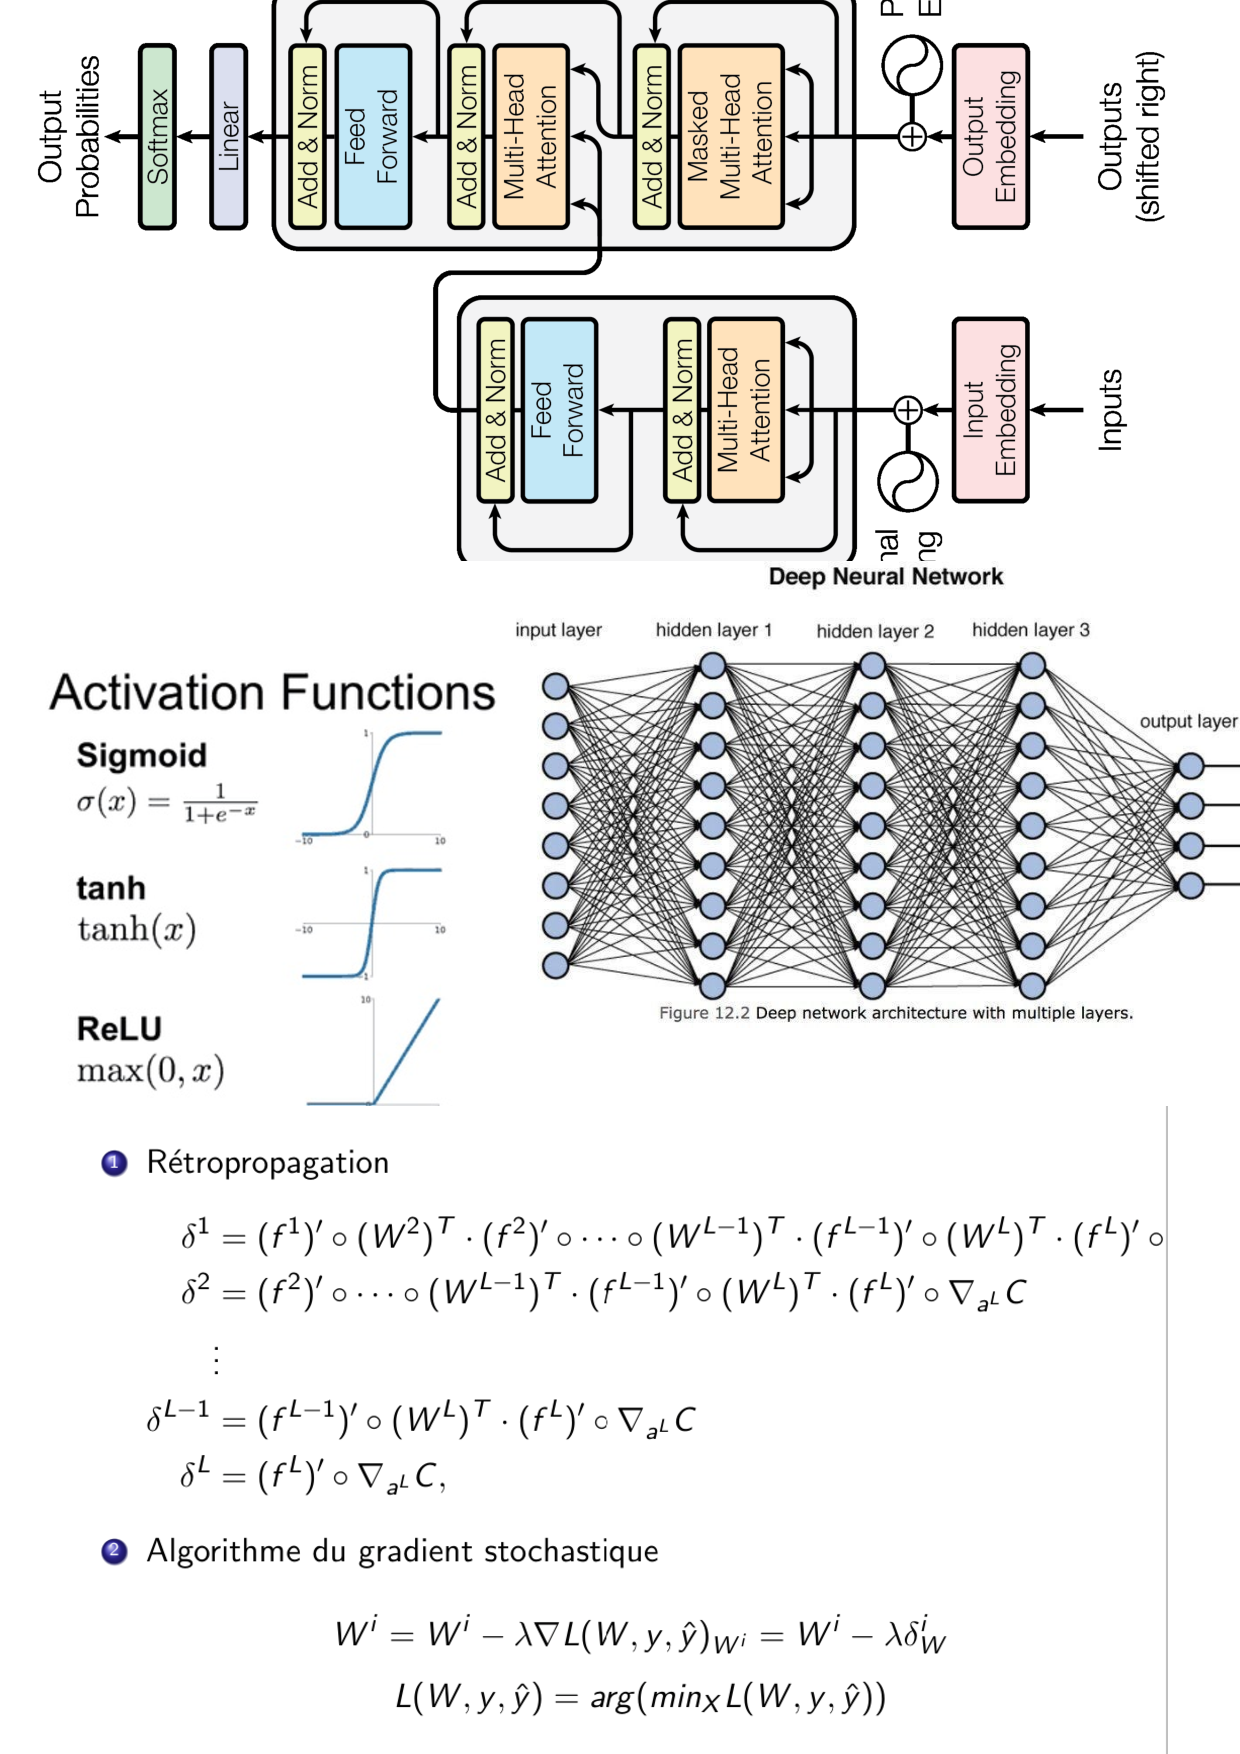
\includegraphics[width=\textwidth]{im}
		\column{.4\textwidth}
		\centering
		\begin{tikzpicture}[node distance=1.5cm,auto]
			\tikzstyle{block} = [rectangle, draw=blue, thick, fill=blue!20,    text width=3.5cm, text centered, rounded corners, minimum height=2em];
			\draw node [block] (cond1){\texttt{Architecture}};
			\draw node [block, below of=cond1] (cond10){\texttt{Metaparamétres}};
			\draw node [block, below of=cond10] (cond2){\texttt{Données (+ nouveaux données)}};
			\draw node [block,below of=cond2](cond3){Apprentissage};
			\draw node [block,below of=cond3](cond4){Fonction $f(X)$};
			
			\draw [draw=blue,thick,->] (cond1)--(cond10);
			\draw [draw=blue,thick,->] (cond10)--(cond2);
			\draw [draw=blue,thick,->] (cond2)--(cond3);
			\draw [draw=blue,thick,->] (cond3)--(cond4);
			\path [draw=blue,thick,<->,loop left,looseness=2] (cond10) edge (cond3);
%			\path [draw=blue,thick,<->,loop left,looseness=2] (cond10) edge (cond1);
			\path [draw=blue,thick,<->,loop left,looseness=2] (cond10) edge node [right] {si besoin} (cond1);
			\path [draw=blue,thick,->] (cond3) -- (cond4) node [midway, right] {si $f(X) = y$};
			
		\end{tikzpicture}
	\end{columns}
\end{frame}

	\begin{frame}
	\begin{center}
{\LARGE Merci pour votre attention }
	\end{center}
\end{frame}



	
\end{document}
